\chapter{PENDAHULUAN}
\pagenumbering{arabic}
\vspace{4ex}
\label{chap:chap1_introduction}

\section{Latar Belakang}
\vspace{1ex}

Permainan dengan basis \textit{Role-Playing Game} (RPG) adalah permainan yang mana pemain memerankan sebuah karakter khusus dalam sebuah cerita. Pada permainan tersebut, pemain memiliki tujuan untuk menjalankan misi dan mengikuti alur cerita dari permainan tersebut sampai selesai. Terdapat berbagai macam variasi jenis dari RPG, salah satunya adalah \textit{turn-based}. Pada \textit{turn-based} RPG, pemain dapat memainkan satu karakter atau lebih yang mana karakter tersebut melakukan serangan secara bergantian antara pemain atau musuh seperti pada Gambar \ref{fig:rpg_turn_based}. Biasanya musuh yang dilawan berupa \textit{Non-Player Character} (NPC).
\vspace{1ex}

\begin{figure} [!h] \centering
	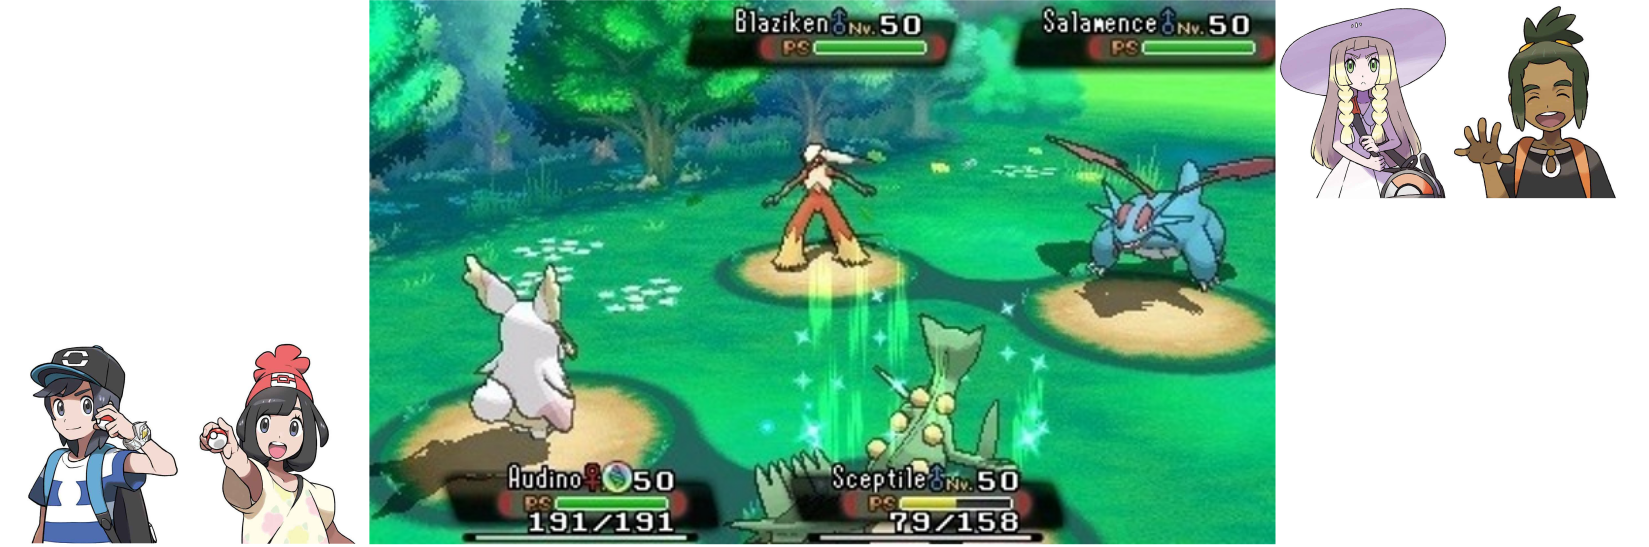
\includegraphics[scale=0.40]{img/turn_based.png}
	\caption{Ilustrasi \textit{Turned-based} RPG}
	\label{fig:rpg_turn_based}
\end{figure}

Pada permainan dengan genre \textit{turn-based} RPG yang terdiri dari banyak karakter baik itu karakter pemain dan musuh. Di mana stats tersebutlah yang akan menentukan jalannya pertarungan antara pemain dan musuh. Kemudian stats juga menunjukan tingkat kesulitan dari musuh, kelemahan dari musuh, daya tahan musuh terhadap serangan dan lain-lain. Hal ini juga merupakan bagian utama dari desain permainan, yang mana nominal pada stats, jumlah pemain dan musuh dapat menentukan beberapa faktor penting lain seperti halnya lamanya permainan dan alur cerita. 
\vspace{1ex}

Banyak penelitian yang mengaplikasikan berbagai bentuk algoritma dan metode untuk mempercepat pembuatan \textit{video games} sepeti halnya pengukuran tingkat kesulitan dengan menggunakan challenging rate (CR) pada permainan 2D \textit{Real Time Strategy} (RTS) \citep{Christyowidiasmoro2016}, pembuatan \textit{game engine} yang berorientasi pada \textit{multi-agent systems} \citep{Marin-Lora2020}, pembuatan level secara otomatis pada permainan secara prosedular dengan tingkat kesulitan tertentu \citep{Wu2018}, ada juga ada yang memakai metode yang dapat menghasilkan \textit{attribute space} untuk menganalisa keseimbangan dalam pertarungan \textit{single unit} pada permainan RTS \citep{Bangay2014}. Berdasarkan beberapa penelitian tersebutlah maka penelitian ini dibuat guna memudahkan desainer permainan dalam mendesain sebuah permainan dengan genre \textit{action} dan \textit{turn-based} RPG.
\vspace{1ex}

Penggunaan berbagai metode seperti $k-$NN, Distribusi Normal dan Naive bayes yang kemudian dilanjutkan dengan diperolehnya data statistik dari untuk pemain dan musuh yang siap digunakan. Kemudian dilanjutkan dengan proses validasi data statistik tersebut apakah sudah sesuai dengan apa yang direncanakan. Pada proses tersebut digunakanlah \textit{Deep Learning} dengan basis \textit{Neural Network} untuk \textit{Multiclass Classification}.
\vspace{1ex}

\section{Rumusan Masalah}
\vspace{1ex}

Pembuatan statistik untuk karakter yang akan dimainkan oleh pemain dan juga karakter musuh pada permainan dengan genre action dan turn-based RPG yang terkadang masih dilakukan secara manual, terlebih lagi jika karakter dari pemain dan musuh pada permainan tersebut sangat banyak maka diperlukannya sebuah program yang mampu menyusun hal tersebut secara otomatis.
\vspace{1ex}

\section{Tujuan}
\vspace{1ex}

Dari permasalahan yang dirumuskan sebelumnya,maka penelitian ini memiliki tujuan sebagai berikut: 

\begin{enumerate}
	\item Mempercepat proses desain permainan dengan menggunakan program yang dapat menghasilkan data statistik untuk karakter dari pemain dan musuh.

	\item Terujinya data statistik untuk karakter pemain dan musuh yang dihasilkan secara otomatis oleh program.
\end{enumerate}

\section{Batasan Masalah}
\vspace{1ex}

Berdasrkan fokus permasalahan pada bagian sebelumnyaa, kemudian diambilah beberapa pembatasa masalah. Berikut adalah batasan-batasan masalah tersebut.

\begin{enumerate}
	\item Data statistik yang dihasilkan oleh program hanya dapat dipakai oleh permainan dengan genre \textit{action} dan \textit{turn-based} RPG.
	
	\item Program yang dibuat untuk menghasilkan data statistik dapat dipakai oleh lebih sama dengan satu karakter pemain dan musuh.

	\item Metode yang digunakan dalam proses pembuatan data statistik pemain dan musuh diantaranya adalah $k-$NN, Normal Distribution dan Naive Bayes.
	
	\item Sedangkan metode yang digunakan untuk menguji tingkat ke validitas dari data yang dibuat tadi digunakanlah metode \textit{deep learning} berbasis \textit{Neural Network} dengan \textit{Multiclass Classification}.
\end{enumerate}

\section{Kontribusi}
\vspace{1ex}

Di harapkan penelitian ini mampu mejadi rujukan dalam proses desain permainan, khususnya saat pembuatan data statistik untuk karakter pemain dan musuh. Selain itu menjadikan para pengembang permainan dengan genre RPG khususnya \textit{action} dan \textit{turn-based} RPG di masa mendatang menjadi lebih cepat.
